\documentclass[a4paper,twoside]{article}
\usepackage{geometry}
\geometry{margin=1cm,vmargin={0pt,1cm}}
\setlength{\topmargin}{-2cm}
\setlength{\paperheight}{23cm}
\setlength{\paperwidth}{18cm}
\setlength{\textheight}{19.6cm}
\setlength{\textwidth}{15cm}
\usepackage{makecell}
%\usepackage{fancyhdr}
\usepackage{siunitx}
\usepackage{amssymb}
\usepackage{indentfirst}
\setlength{\parindent}{0.5em}

\pagenumbering{arabic} 
\usepackage{pdfpages}
% useful packages.

\usepackage{ctex}

\usepackage{color}
\usepackage{multirow}
\usepackage{caption}
\usepackage{mathrsfs}
 \usepackage{amsfonts}
\usepackage{amsmath}
\usepackage{amsthm}
\usepackage{enumerate}
\usepackage{xcolor,graphicx,float,subfigure}
\usepackage{epstopdf}
\usepackage{multicol}
\usepackage{fancyhdr}
\usepackage{layout}
\usepackage{listings}
\usepackage{dsfont}
\lstset{language=Matlab}
\lstset{breaklines}
\lstset{extendedchars=false}
\usepackage[colorlinks,linkcolor=blue]{hyperref}
\usepackage{xcolor}
%\usepackage{cite}
%\usepackage[numbers,sort&compress]{natbib} 
%\setcitestyle{open={},close={}}
%\usepackage{natbibspacing}
%\renewcommand{\refname}{}
\usepackage{anyfontsize}

\usepackage{tikz}
\usetikzlibrary{calc}
\usetikzlibrary{arrows.meta}
\tikzset{
  dot/.style={
    circle, fill=black, inner sep=1pt, outer sep=0pt
  },
  dot label/.style={
    circle, inner sep=0pt, outer sep=1pt
  }
  arrow1/.style = {
    draw = black, thick, -{Latex[length = 4mm, width = 1.5mm]},
  }
}


% -------------------
% Theorem Environments
% -------------------
\theoremstyle{definition}
\newtheorem{thm}{Theorem}[section]
\newtheorem{prop}{Proposition}[section]
\newtheorem{lem}{Lemma}[section]
\newtheorem{coro}{Corollary}[section]

\newtheorem{exm}{Example}[section]
\newtheorem{nex}{Non-Example}[section]
\newtheorem{defn}{Definition}[section]
\theoremstyle{remark}
\newtheorem{rmk}{Remark}[section] 
\numberwithin{equation}{section}


\newcommand{\dif}{\mathrm{d}}
\newcommand{\avg}[1]{\left\langle #1 \right\rangle}
\newcommand{\difFrac}[2]{\frac{\dif #1}{\dif #2}}
\newcommand{\pdfFrac}[2]{\frac{\partial #1}{\partial #2}}
\newcommand{\OFL}{\mathrm{OFL}}
\newcommand{\UFL}{\mathrm{UFL}}
\newcommand{\fl}{\mathrm{fl}}
\newcommand{\op}{\odot}
\newcommand{\Eabs}{E_{\mathrm{abs}}}
\newcommand{\Erel}{E_{\mathrm{rel}}}

\newcommand{\Zero}{\hat{0}}
\newcommand{\One}{\hat{1}}
\newcommand{\Int}{\mathrm{int}}
\newcommand{\unitV}{\mathds{1}}

\newcommand{\bmi}{\mathbf{i}}
\newcommand{\bmj}{\mathbf{j}}
\newcommand{\bmn}{\mathbf{n}}

\newcommand{\dist}[2]{\text{dist}\left(#1, #2\right)}
\newcommand{\scientific}[2]{#1 \times 10^{#2}}


%\newcommand{\Dim}{{\mathbf{D}}}
\newcommand{\Dim}{{\scriptsize \textsf{D}}}
\newcommand{\me}{\mathrm{e}}
\newcommand{\mi}{\mathrm{i}}

%\newcommand{\mod}{\mathrm{mod}}
\newcommand{\curve}[1]{\widetilde{#1}}
%\newcommand{\dt}{\delta t}
\newcommand{\dt}{\tau}
\newcommand{\isCovered}{\mathbin{ < \! \! \! \! \cdot }}
%\newcommand{\cIncluded}{\mathbin{ \prec \! \! \! \cdot }}
\newcommand{\coveredBy}{\lhd}
%\newcommand{\regrz}[1]{\mathrm{cl}\left(\mathrm{int}\left(#1\right)\right)}
\newcommand{\regrz}[1]{\mathrm{reg}\left(#1\right)}
%\newcommand{\sgncup}{\ \hat{\cup} \ }
\newcommand{\Span}{\mathrm{span}}
\newcommand{\timeline}[2]{\phi_{t_0}^{#1}\left( #2 \right)}
\newcommand{\timeBP}[1]{\overleftarrow{#1}}
\newcommand{\timeBPA}[1]{\mathring{\overleftarrow{#1}}}
\newcommand{\streak}[2]{\Psi_{t_0}^{#1}\left(#2\right)}
\newcommand{\timelineA}[2]{\mathring{\phi}_{t_0,#2}^{#1}}
\newcommand{\DRLN}[1]{{\cal D}_{\curve{#1}}}
\newcommand{\DRLLN}[1]{{\cal D}_{\overline{#1}}}
\newcommand{\DRLNA}[1]{\mathring{\cal D}_{\curve{#1}}}
%\newcommand{\oplusDR}{\,\overline{\oplus}\,}
\newcommand{\oplusDR}{\,\bar{\oplus}\,}
\newcommand{\qo}{\hat{q}}
\newcommand{\xo}{\hat{x}}
\newcommand{\yo}{\hat{y}}
\newcommand{\closure}[1]{\textrm{cl}\left(#1\right)}
\newcommand{\vertexSequence}[4]{
  \left( #1 \rightarrow #2 \rightarrow #3 \rightarrow #4 \rightarrow #1\right)}

\newcommand{\ppSpace}{\Pi_{<\kappa,\bm{\xi},\bm{\nu}}}
\newcommand{\pnSpace}{\mathbb{P}_{<\kappa}}
\newcommand{\pnSpaceK}[1]{\mathbb{P}_{#1}}

\newcommand{\Pyr}[2]{\textrm{Pyr}_{\cal{#1}}\left(\mathbf{#2}\right)}

\let\OldTexttt\texttt
\renewcommand{\texttt}[1]{{\color{blue} \OldTexttt{#1}}}

%\pagestyle{plain}
\pagestyle{fancy}
\fancyhf{}
\fancyhead[LE,RO]{\textbf{\thepage}}

\makeatletter
\newcommand\sixteen{\@setfontsize\sixteen{17pt}{6}}
\renewcommand{\maketitle}{\bgroup\setlength{\parindent}{0pt}
\begin{flushleft}
\sixteen\bfseries \@title
\medskip
\end{flushleft}
\textit{\@author}
\egroup}
\makeatother


\title{Efficient C++}

\begin{document}
\maketitle
\tableofcontents

\newpage
\section{Accustoming yourself to C++}

\subsection{Prefer \texttt{const, enum, inline} to \texttt{\#define}}
\label{sec:Item-2}
\begin{itemize}
\item \texttt{\#define} will be confusing if you get an error during
  complication.
\item Use of \texttt{constant} yield smaller code than using a
  \texttt{\#define}.
\end{itemize}

When replacing \texttt{\#defines} with constants, there are two
spectial cases:
\begin{itemize}
\item Defining constant pointers'': \texttt{const char* const
    authorName = "xxx''}
\item Concerning class-specific constants. To limit the scope od a
  constant to a class, you must make it a member, to ensure there is
  at most one copy of the constant, you must make it a \texttt{static}
  member.
\begin{verbatim}
class Game{
private:
  static const int Nums = 5;
  int scores[Nums];
  ...
};
\end{verbatim}
  If it is an integral type (integers, chars, bools), we do not need
  provide a definition. Otherwise we need a separate definition in
  \textbf{implementation file}:
\begin{verbatim}
const int Game::Nums; // definition of Nums, no initial value here.
\end{verbatim}
  There is no way to carete a class-specific constant using a
  \texttt{\#define}.

 
\item  In another way, we can use "enum hack'':
  \begin{verbatim}
class Game{
private:
  enum {Nums = 5};
  int scores[Nums];
  ...
};
\end{verbatim}
  \begin{itemize}
  \item The enum hack behaves in some ways more like a \texttt{\#define},
  for example, it's legal to take the address of a const but not to an
  enum. 
\item Also, enums never result in unnecessary memory
  allocation. 
\item the enum hack is a fundamental technique of template
  metaprogramming. (see Section \ref{sec:Item-48})
  \end{itemize}
\end{itemize}

Another common misuse of the \texttt{\#define} is using it to
implement macros that look like functions but that do not incur the
overhead of a function call. For example:
\begin{verbatim}
#define CALL_WITH_MAX(a,b) f( (a) > (b) ? (a) : (b) )
\end{verbatim}

You have to remember to parenthesize all the arguments in the macro
body. Oherwise you will run into trouble. However, even you get that
right, the weird things can happen:
\begin{verbatim}
int a = 5, b = 0;
CALL_WITH_MAX(++a, b);    // a is incremented twice
CALL_WITH_MAX(++a, b+10); // a is incremented once
\end{verbatim}

Now we can use a template for an inline function in Section \ref{sec:Item-30}
\begin{verbatim}
template <class T>
inline void callWithMax(const T& a, const T &b){
  f(a > b ? a : b);
} // because we donot know what T is, we pass by reference-to-const.
\end{verbatim}

\subsection{Use \texttt{const} whenever possible}
\label{sec:Item-3}
The \texttt{const} keyword is remarkably versatile. For pointers, you
can specify whethwe the pointer itself is const or the data is const:
\begin{verbatim}
char greeting[] = "Heello";
const char *p = greeting;  //non-const pointer, const data
char *const p = greeting;  //const pointer, non-const data
const std::vector<int>::iterator iter = vec.begin(); // iter acts like a T *const;
++ iter;  // error! iter is const.
std::vector<int>::const_iterator cIter = vec.begin(); // iter acts like a const T*
*cIter = 10; // error! *cIter is const.
\end{verbatim}

Some of the most powerful uses of \texttt{const} stem from its
application to function declarations:

\begin{itemize}
\item \textbf{Having a function return a constant value} sometimes can reduce
  the incidence of the clinent errors without giving up safety or
  efficiency. For example: In Section \ref{sec:Item-24}
\begin{verbatim}
const Rational operator*(const Rational &lhs, const Rational &rhs);
\end{verbatim}
  We can avoid the unintentional error like \texttt{if(a * b = c)}.
  Such code would be illegal if a and b were of a built-in
  type. \textbf{ One of the hallmarks of good user-defined types is
    that they avoid gratuitous incompatibilities with built-in types.}
  (see Section \ref{sec:Item-18})
\item The purpose of \textbf{const on member functions} is to identify
  which member functions may be invoked on \texttt{const} objects,
  which are important for two reasons:
  \begin{itemize}
  \item They make the interface of a class easier to understand. It is
    important to know which functions may modify an object.
  \item They make it possible to work with \texttt{const}
    objects. There is a fundamental ways to improve performance, which
    is \textbf{pass objects by reference-to-const}, which will
    explains in Section \ref{sec:Item-20}.
  \end{itemize}
\item \textbf{Member functions differing only in \texttt{constness}}
  can be overloaded, which is an important feature of C++. For
  example:
\begin{verbatim}
class TextBlock{
public:
  const char &operator[](std::size_t position) const;
  char &operator[](std::size_t position);
};
\end{verbatim}
By overloading and giving the different versions different return
types, you can have \texttt{const} and non-\texttt{const} TextBlocks
handled differently.
\item There are two prevailing notions of \texttt{const}:
  \textbf{bitwise const} and \textbf{logical const}. Bitwise constness
  is easy to understand, for logical constness, here is an example''
\begin{verbatim}
class CTextBlock{
public:
  std::size_t length() const;
private:
  char *pText;
  std::size_t textLength;
  bool lengthIsValid;
};
std::size_t CTextBlock::length() const{
  if(!lengthIsValid){
    textLength = std::strlen(pText); // error!
    lengthIsValid = true;   // error!
  }
  return textLength;
}
\end{verbatim}
Now the solution is simple: \texttt{mutable} frees non-static data
members from the constraints of bitwise constness.

\item \textbf{Avoiding Duplication in \texttt{const} and
    \texttt{non-const} member functions}. Sometimes
  \texttt{operator[]} in \texttt{TextBlock} not only returns a
  reference to the character, it also performed bounds checking,
  logged access information, etc. Putting all this in both functions
  yields more compilation time, maintenance and code-bloat. It is
  possible to move all codes into a seperate member function
  (private).

  There is an another way. That is, you want to have one version of
  \texttt{operator[]} call the other one.
\begin{verbatim}
class TextBolock{
public:
  ...
  const char &operator[](std::size_t position) const{ ... }
  char &operator[](std::size_t position){
    return const_cast<char&>(static_cast<const TextBlock&>(*this)[position]);
  }
\end{verbatim}
  The one that removes \texttt{const} can be accomplished only via
  \texttt{const\_cast}. Though casting is such a bad idea as a general
  rule (see \ref{sec:Item-27}), but code duplication is no picnic
  either. It is determined by you, but this technique is worth knowing.
\end{itemize}

\subsection{Make sure that objects are initialized before they are used}
\label{sec:Item-4}

If you are in the C part of C++ and initialization would probably
incur a runtime cost, initialization is not guaranteed to take
place. This explains why array (from C part of C++) isn't necessarily
guaranteed to have its contents initialized but a vector is.
The best way is to \textbf{always initialize objects before you use
  them.}


\begin{itemize}
\item For built-in types, you need to do this manually, for else,
the responsibility for initialization falls on constructors. However,
\textbf{do not confuse assignment with initialization.}
\begin{verbatim}
class ABEntry{
public:
  ABEntry(const std::string &name, const stdLLstring &address);
private:
  std::string theName;
  std::string theAddress;
  int numTimesConsulted;
};
ABEntry::ABEntry(const std::string &name, const std::string &address){
  theName = name;          \\ these are all assignments, not initializations.
  theAddress = address;
  numTimesConsulted = 0;
}
\end{verbatim}
Their default constructors were automatically called prior to entering
the ABEntry constructor. But this is not true for numTimesConsulted
because it is a built-in type. For it, there is no guarantee it was
initialized at all prior to its assignment.

A better way is to use the member initialization list instead of
assignments:
\begin{verbatim}
ABEntry::ABEntry(const std::string &name, const std::string &address)
: theName(name), theAddress(address), numTimesConsulted(0)
{} // these are now all initializations.
\end{verbatim}
It is more efficient because default consturctions were wasted before.

For objects of built-in type, ifor consistency, it is often best to
initialize everthing via member initialization. There is a policy of
\textbf{always listing every data member on the initialization list}.
\begin{verbatim}
ABEntry::ABEntry(): theName(), theAddress(), numTimesConsulted(0)
{}
\end{verbatim}
Sometimes initialization list must be used for built-in types. For
example: data members that are \texttt{const} or \texttt{references}
that must be initialized. (See \ref{sec:Item-5}).

When class has multiple constructors, we can omit entries in the lists
for data members where assignment works as well as true
initialization, moving the assignments to a single function that all
constructors call.

One aspect of C++ that is not fickle is \textbf{the order in which an
  object's data is initialized}. This order is always the same: base
classes, derived clasees, data members in the order in which they are
declared. (\textbf{When initialize an array, declare the size first.})

\item \textbf{The order of initialization of non-local static objects difined
    in different translation units} is important.

  A \textbf{\texttt{static} object} is one that exists from the time it's
  constructed until the end of the program, including global objects,
  objects declared \texttt{static} inside classes, functions or at
  file scope. \texttt{Static} objects inside functions are known as
  local static objects.

  If initialization of a non-local static object in one translation
  unit uses a non-local static object in a different translation unit,
  \textbf{the object it uses could be uninitialized.} For example, 
\begin{verbatim}
class FileSystem{
public:
  std::size_t numDisks() const;
  ...
};
extern FileSystem tfs;
\end{verbatim}
  In another file, there is
\begin{verbatim}
class Directory{
public:
  Directory(params);
  ...
};
Directory::Directory(params){ 
  std::size_t disks = tfs.numDisks(); 
  ...
}
\end{verbatim}
Further suppose the client decides to create a single Diretory object \texttt{tempDir},
\texttt{tfs} and \texttt{tempDir} are created by different people at
different times in different source files. How can you be sure that
\texttt{tfs} will be initialized before \texttt{tempDir}? You can't
because \textbf{the relatice order of initilization of non-local
  static objects defined in different translation units is undefined.}

Fortunately, a small design change eliminates the problem
entirely. All that has to be done is to \textbf{move each non-local
  static object into its own function, where it's declared
  \texttt{static}}. This approach is founded on C++'s guarantee that local
static objects are initilized when the object's definition is first
encountered during a call to that function.
\begin{verbatim}
FileSystem &tfs(){
  static FileSystem fs;
  return fs;
}
Directory &tempDir(){
  static Directory td(params);
  return td;
}
\end{verbatim}
The reference-returning functions dictated by this scheme are always
simple, which makes them excellent candidates for inlining. On the
other hand, it make them problematic in multithreaded systems. One way
to deal with it is to invoke all the reference-returning functions
during the single-threaded startup portion of the program.
\end{itemize}

To avoid using objects before they are initialized, you need to do
three things:
\begin{itemize}
\item manually initialize non-member objects of built-in types
\item use member initialization lists to initialize all parts of an
  object
\item design around the initialization order uncertainty that afflicts
  non-local static objects defined in separate translation units.
\end{itemize}

\newpage
\section{Constructors, destructors, assignment operators}

\subsection{Know what functions C++ silently writes and calls}
\label{sec:Item-5}

Compilers will declare their own versions of a copy constructor, copy
assignment, destructor if you don't declare them. Further more, if you
declare no constructors, compliers will also declare a default
constructor. All these functions are \texttt{public and inline} (See
\ref{sec:Item-30}).
\begin{verbatim}
class Empty
public:
  Empty() { ... } // default constructor
  Empty(const Empty& rhs) { ... } // copy constructor
  ~Empty() { ... } // destructor — see below for whether it’s virtual
  Empty& operator=(const Empty& rhs) { ... } // copy assignment operator
};
\end{verbatim}
\begin{itemize}
\item The generated destructor is \textbf{non-virtual} (See \ref{sec:Item-7})
  unless it's for a class inheriting from a base class that declares a
  virtual destructor,
\item The copy constructor and assignment simply copy each non-static
  data member.
\item If you want to support copy assignment in a class \textbf{containing a
  reference or const member}, you must define the copy assignment
  operator yourself.
\item Compilers reject implicit copy assignment operators in derived
  classes that inherit from \textbf{base classes declaring the copy assignment
  operator \texttt{private}}.
\end{itemize}

\subsection{Explicitly disallow the use of compilergenerated functions
  you do not want.}
\label{sec:Item-6}

Use \texttt{=delete} or declare \texttt{private} and give no
implementations if you don't want a class to support a particular
kind of copy functionality.

\subsection{Declare destructors virtual in polymorphic base classes.}
\label{sec:Item-7}

A particluar example is get function of a factory, we will get a
pointer to a base class. If we declare destructors non-virtual, \textbf{the
  object will be partially destroyed}.

\begin{itemize}
\item If a class does not contain virtual functions, that often indicates it is
not meant to be used as a base class, so making the
destructor virtual is usually a bad idea because the size of the
class will increase. \textbf{Declare a virtual destructor in a
class if and only if that class contains at least one virtual function.}
\item The implementation of virtual functions requires that objects carry
information that can be used at runtime to determine which virtual
functions should be invoked on the object. This information typically
takes the form of a pointer called a \texttt{vptr}. The
\texttt{vptr} points to an array of function pointers called a
\texttt{vtbl}; each class with virtual functions has an associated
\texttt{vtbl}. When a virtual function is invoked on an object, the
actual function called is determined by following the object's
\texttt{vptr} to a \texttt{vtbl} and then looking up the appropriate
function pointer in the \texttt{vtbl}. 
\item Not all base classes are designed to be used polymorphically. \textbf{Neither
the standard string type, for example, nor the STL container types are
designed to be base classes at all,} much less polymorphic ones.
\item If we want an abstract base class, we can declare a pure virtual
  destructor, but \textbf{we must provide a definition for the pure
    virtual destructor.}
\end{itemize}

\subsection{Prevent exceptions from leaving destructors}
\label{sec:Item-8}

\begin{itemize}
\item  Destructors should never emit exceptions. If functions called in a
destructor may throw, the destructor should catch any exceptions,
then swallow them or terminate the program.
\item If class clients need to be able to react to exceptions thrown during
an operation, the class should provide a regular (i.e.,
non-destructor) function that performs the operation.
\end{itemize}


\subsection{Never call virtual functions during construction or
  destruction}
\label{sec:Item-9}

\begin{itemize}
\item \textbf{During base class construction of a derived class object, the
  type of the object is that of the base class.}  Not only do virtual
functions resolve to the base class, but the
parts of the language using runtime type information (e.g.,
\texttt{dynamic\_cast} (see \ref{sec:Item-27}) and \texttt{typeid})
treat the object as a base class type.
\item The same reasoning applies during destruction.
\item It's not always so easy to detect calls to virtual functions
  during construction or destruction.
\begin{verbatim}
class Transaction {
public:
  Transaction() { init(); } // call to non-virtual...
  virtual void logTransaction() const = 0;
  ...
private:
void init() {
  ...
  logTransaction(); // ...that calls a virtual!
}
};
\end{verbatim}
\end{itemize}

\subsection{Have assignment operators return a reference to
  \texttt{*this}}
\label{sec:Item-10}

One of the interesting things about assignments is that you can chain
them together:
\begin{verbatim}
int x, y, z;
x = y = z = 15; // chain of assignments.
x = (y = (z = 15)); //equivalent.
\end{verbatim}

The way this is implemented is that \textbf{assignment returns a
  reference to its left-hand argument}. This convention applies to all
assignment operators.

\begin{verbatim}
class Widget {
public:
  ...
  Widget &operator=(const Widget &rhs){
    ...
    return *this;
  }
  Widget& operator+=(const Widget& rhs) // the convention applies to 
  {                                     // +=, -=, *=, etc.
    ...
    return *this;
  }
Widget& operator=(int rhs)              // it applies even if the
  {                                     // operator’s parameter type
  ...                                   // is unconventional
  return *this;
  }
};
\end{verbatim}

\subsection{Handle assignment to self in \texttt{operator=}}
\label{sec:Item-11}

If you follow the advice of \ref{sec:Item-13} and \ref{sec:Item-14},
you'll always use objects to  manage resources, and you'll make sure
that the resource-managing objects behave well when copied.

If you try to manage resources yourself, however (which you'd
certainly have to do if you were writing a resourcemanaging class),
you can fall into the trap of \textbf{accidentally releasing a
  resource} before you're done using it. For example,
\begin{verbatim}
Widget& Widget::operator=(const Widget& rhs) // unsafe impl. of operator=
{
  delete pb; // stop using current bitmap
  pb = new Bitmap(*rhs.pb);                  // start using a copy of rhs’s bitmap
  return *this;                              
}
\end{verbatim}

Now, the self-assignment problem here is that itself holds a pointer
to a deleted object! There are three ways to prevent this error.

\begin{itemize}
\item check for assignment to self via an identity test at the top of
  \texttt{operator=}.
\begin{verbatim}
Widget& Widget::operator=(const Widget& rhs){
  if (this == &rhs) return *this; // identity test: if a self-assignment, do nothing
  delete pb;
  pb = new Bitmap(*rhs.pb);
  return *this;
}
\end{verbatim}
  This works but there is also exception-unsafe. If the "new Bitmap''
  expression yields an exception (either because there is insufficient
  memory for the allocation or because Bitmap's copy constructor
  throws one), the Widget will end up holding a pointer to a deleted
  Bitmap.  You can't safely delete them. You can't even safely read them.

\item  \ref{sec:Item-29} explores exception safety in depth,
but in this Item, it suffices to observe that in many cases, a careful
ordering of statements can yield exception-safe code.
\begin{verbatim}
Widget& Widget::operator=(const Widget& rhs)
{
  Bitmap *pOrig = pb; // remember original pb
  pb = new Bitmap(*rhs.pb); // point pb to a copy of rhs’s bitmap
  delete pOrig; // delete the original pb
  return *this;
}
\end{verbatim}
Now, if "\texttt{new Bitmap}'' throws an exception, \texttt{pb}
remains unchanged. 
\item If you're concerned about efficiency, use the technique known as
  "\textbf{copy and swap}'', which is described in \ref{sec:Item-29}.
\begin{verbatim}
class Widget {
  ...
  void swap(Widget& rhs); // exchange *this’s and rhs’s data, see Item 29 for details
};
Widget& Widget::operator=(const Widget& rhs){
  Widget temp(rhs); // make a copy of rhs’s data
  swap(temp); // swap *this’s data with the copy’s
  return *this;
}
\end{verbatim}
\item Make sure that any function operating on more than one object
  behaves correctly if two or more of the objects are the same.
\end{itemize}

\subsection{Copy all parts of an object}
\label{sec:Item-12}

When you're writing a copying function, be sure to
\begin{itemize}
\item copy \textbf{all} local data members,
\begin{verbatim}
class Customer {
public:
  ...
  Customer(const Customer& rhs);
  Customer& operator=(const Customer& rhs);
  ...
private:
  std::string name;
  Date lastTransaction;
};

Customer::Customer(const Customer& rhs)
: name(rhs.name){} // copy rhs’s data  Data has been forgotten!!!

Customer& Customer::operator=(const Customer& rhs)
{
  name = rhs.name; // copy rhs’s data
  return *this;    //  DATE!
}
\end{verbatim}
\item invoke the appropriate copying function in \textbf{all base
    classes}.
\begin{verbatim}
class PriorityCustomer: public Customer { // a derived class
public:
  ...
  PriorityCustomer(const PriorityCustomer& rhs);
  PriorityCustomer& operator=(const PriorityCustomer& rhs);
  ...
private:
  int priority;
};
PriorityCustomer::PriorityCustomer(const PriorityCustomer& rhs)
: Customer(rhs), // invoke base class copy ctor
  priority(rhs.priority){}
PriorityCustomer&
PriorityCustomer::operator=(const PriorityCustomer& rhs)
{
  Customer::operator=(rhs); // assign base class parts
  priority = rhs.priority;
  return *this;
}
\end{verbatim}
\item if you find that your copy constructor and copy assignment
operator have similar code bodies, \textbf{eliminate the duplication by
creating a third member function that both call}.
\end{itemize}

\clearpage
\section{Resource Management}

This chapter begins with a straightforward object-based approach to
resource management built on C++'s support for constructors,
destructors, and copying operations. Experience has shown that
disciplined adherence to this approach can all but eliminate resource
management problems. The chapter then moves on to Items dedicated
specifically to memory management. These latter Items complement
the more general Items that come earlier, because objects that manage
memory have to know how to do it properly.

\subsection{Use objects to manage resources}
\label{sec:Item-13}

To make sure that the resource  is always released, we need to put
that resource inside an object whose destructor will automatically
release the resource when control leaves domain.
\begin{verbatim}
void f(){
  std::auto_ptr<Investment> pInv(createInvestment()); // call factory function
   ... 
} // automatically delete pInv via auto_ptr’s dtor
\end{verbatim}

This simple example demonstrates the two critical aspects of using
objects to manage resources:
\begin{itemize}
\item \textbf{Resources are acquired and immediately turned over to
  resource-managing objects}: the resource returned by
  \texttt{createInvestment} 
  is used to initialize the \texttt{auto\_ptr} that will manage it. In 
fact, the idea of using objects to manage resources is often called
\textbf{Resource Acquisition Is Initialization (RAII)}.
\item \textbf{Resource-managing objects use their destructors to ensure
that resources are released}.
\end{itemize}

See more details of smart pointers in Section \ref{sec:SmartPointer}.
\textbf{Pay attention to smart pointer to aynamically allocated arrays.}

If you need to craft your own resource-managing
classes, that's not terribly difficult to do, but it does need to
consider of Section \ref{sec:Item-14} and \ref{sec:Item-15}.

\subsection{Think carefully about copying behavior in
  resource-managing classes.}
\label{sec:Item-14}

What should happen when an RAII object is copied? Most of the time,
you'll want to choose one of the following possibilities:

\begin{itemize}
\item \textbf{Prohibit copying}: declare the copying operations
  private.
\item \textbf{Reference-count the underlying resource}: See
  \texttt{shared\_ptr}.
\item \textbf{Copy the underlying resource}: copying a
  resource-managing object performs a "deep copy''.
\item \textbf{Transfer ownership of the underlying resource}: See \texttt{unique\_ptr}.
\end{itemize}

\subsection{Provide access to raw resources in resource-managing classes. }
\label{sec:Item-15}

In a perfect world, you'd rely on such classes for all your
interactions with resources, never sullying your hands with direct
access to raw resources. But the world is not perfect. There are two
general ways to do it: \textbf{explicit conversion } and
\textbf{implicit conversion}.

\begin{itemize}
\item \texttt{shared\_ptr} and \texttt{unique\_ptr} both offer a get
  member function to perform an \textbf{explicit conversion}, i.e., to return
  (a copy of) the raw pointer inside the smart pointer object.
\begin{verbatim}
FontHandle getFont(); // from C API — params omitted for simplicity
void releaseFont(FontHandle fh); // from the same C API

class Font { // RAII class
public:
  explicit Font(FontHandle fh) // acquire resource; use pass-by-value,because the C API does
  : f(fh){}
  ~Font() { releaseFont(f ); } // release resource
  FontHandle get() const { return f; } // explicit conversion function
  ... // handle copying (see Item 14)
private:
  FontHandle f; // the raw font resource
};
\end{verbatim}
\item However, sometimes we might find the need to explicitly request
  such conversions off-putting enough to avoid using the class . That,
  in turn,would increase the chances of leaking fonts.
\item The alternative is to have \texttt{Font} offer an implicit conversion
  function to its \texttt{FontHandle}, which  makes calling into the C
  API easy and natural:
\begin{verbatim}
class Font {
public:
  operator FontHandle() const // implicit conversion function
  { return f; }
  ...
};
\end{verbatim}
\item The downside is that implicit conversions increase the chance of
errors. For example, a client might \textbf{accidently} create a
\texttt{FontHandle} when a \texttt{Font} was intended:
\begin{verbatim}
Font f1(getFont());
FontHandle f2 = f1;
\end{verbatim}
When \texttt{f1} is destroyed, the font will bereleased, and
\texttt{f2} will dangle.
\end{itemize}

In general, explicit conversion is safer, but implicit conversion is
more convenient for clients.

It may have occurred to you that functions returning the raw resource
inside an RAII class are \textbf{contrary to encapsulation}.  That's
true, but it's not the design disaster it may at first appear, it
hides what clients don't need to see, but it makes available those
things that clients honestly need to access.

\subsection{Use the same form in corresponding uses of new and delete}
\label{sec:Item-16}

\begin{verbatim}
std::string *stringArray = new std::string[100];
...
delete stringArray;
\end{verbatim}

At the very least, 99 of the 100 string objects pointed to by stringArray
are unlikely to be properly destroyed, because \textbf{their
  destructors will probably never be called}.

The memory layout for single objects is generally different
from the memory layout for arrays. In particular, the memory for an
array usually includes the size of the array, thus making it easy for
delete to know how many destructors to call.

\begin{figure}[H]
  \centering
  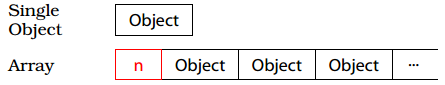
\includegraphics[width = 0.5\textwidth]{ArrayMemLayout.png}
\end{figure}

The rule is simple: if you use [] in a \texttt{new} expression, you
must use [] in the corresponding \texttt{delete} expression. If you
don't use [] in a \texttt{new} expression, don't use [] in the
matching \texttt{delete} expression.

\subsection{Store newed objects in smart pointers in standalone statements.}
\label{sec:Item-17}

Suppose we have a function to reveal our processing priority and a
second function to do some processing on a dynamically allocated
Widget in accord with a priority:

\begin{verbatim}
int priority();
void processWidget(std::tr1::shared_ptr<Widget> pw, int priority);
\end{verbatim}

Consider now a call to \texttt{processWidget}:
\begin{verbatim}
processWidget(new Widget, priority());
\end{verbatim}

It won't compile. \texttt{shared\_ptr'}s constructor taking a raw
pointer is \texttt{explicit}, so there's no implicit conversion. The
following code, however, will compile: 
\begin{verbatim}
processWidget(shared_ptr<Widget>(new Widget), priority());
\end{verbatim}

Although we're using object-managing resources everywhere here,
\textbf{this call may leak resources}.

Before \texttt{processWidget} can be called, then, compilers must generate
code to do these three things:
\begin{itemize}
\item Call \texttt{priority}
\item Execute \texttt{new Widget}
\item Call the \texttt{shared\_ptr} constructor
\end{itemize}

If \texttt{new Widget} expression executed before \texttt{priority()},
and  the call to \texttt{priority()} yields an exception, the pointer
returned from \texttt{new Widget} will be lost.

The way to avoid problems like this is simple: use a separate
statement to create the \texttt{Widget} and store it in a smart pointer, then
pass the smart pointer to \texttt{processWidget}:

\begin{verbatim}
std::tr1::shared_ptr<Widget> pw(new Widget); 
processWidget(pw, priority());
\end{verbatim}

\clearpage
\section{Designs and Declarations}


\clearpage
\section{Appendix}

\subsection{智能指针}
\label{sec:SmartPointer}
\texttt{shared\_ptr}使用了引用计数(use count)技术,当复制个
\texttt{shared\_ptr}对象时,被管理的资源并没有被复制,而是增加了引用计
数。当析 构一个\texttt{shared\_ptr}对象时,也不会直接释放被管理的的资
源,而是将引用计数减一。当引用计数为0时,才会真正的释放资源。
\texttt{shared\_ptr}可以方便的共享资源而不必创建多个资源。

\texttt{unique\_ptr}则不同。\texttt{unique\_ptr}独占资源,不能拷贝,只
能移动。移动过后的\texttt{unique\_ptr}实例不再占有资源。当
\texttt{unique\_ptr}被析构时,会释放所持有的资源。
\begin{verbatim}
unique_ptr<T> b = std::move(a);
\end{verbatim}
\texttt{weak\_ptr}可以解决\texttt{shared\_ptr}所持有的资源循环引用问题。
\texttt{weak\_ptr}在指向\texttt{shared\_ptr}时,并不会增加
\texttt{shared\_ptr}的引用计数。所以\texttt{weak\_ptr}并不知道
\texttt{shared\_ptr}所持有的资源是否已经被释放。这就要求在使用
\texttt{weak\_ptr}获取\texttt{shared\_ptr}时需要判断
\texttt{shared\_ptr}是否有效。

\begin{verbatim}
struct Boo;
struct Foo{
    std::shared_ptr<Boo> boo;
};
struct Boo{
    std::shared_ptr<Foo> foo;
};
\end{verbatim}

\texttt{Foo}中有一个智能指针指向\texttt{Goo},而\texttt{Goo}中也有一根
智能指针指向\texttt{Foo},这就是循环引用,我们可以使用
\texttt{weak\_ptr}来解决这个问题。

关于智能指针的一些tips:
\begin{itemize}
\item 智能指针抛开类型T,是线程安全的,因为智能指针底层使用的引用计数是
\texttt{atomic}的原子变量,原子变量在自增自减时是线程安全的,这保证了
多线程读写智能指针时是安全的。
\item 尽可能不要使用裸指针初始化智能指针,因为可能存在同一个裸指针初始
  了多个智能指针,在智能指针析构时会造成资源的多次释放。
\item 不要从智能指针中使用\texttt{get}函数返回裸指针去为另一个智能指针
  赋值,因为如果返回的裸指针被释放了,智能指针持有的资源也失效了,对智
  能指针的操作是未定义的行为。
\item \texttt{shared\_ptr}和\texttt{unique\_ptr}都可以用\texttt{reset}
  函数来释放智能指针,但\texttt{shared\_ptr}没有\texttt{release}函数,
  \texttt{unique\_ptr}的\texttt{release}函数会返回内置指针,并将自身置
  为空。
\item 与\texttt{uniqu\_ptr}不同,删除器不是\texttt{shared\_ptr}类型的
  组成部分。假设,\texttt{shared\_ptr<T> sp2(q,deleter2)},尽管
  \texttt{sp1}和\texttt{sp2}有着不同的删除器,但两者的类型是一致的,都
  可以被放入\texttt{vector<shared\_ptr<T>>}类型的同一容器里。
\item 与\texttt{std::unique\_ptr}不同,自定义删除器不会改变
  \texttt{std::shared\_ptr}的大小。其始终是祼指针大小的两倍。
\item \texttt{shread\_ptr}和\texttt{unique\_ptr}都可以持有数组,但是这
  里需要在\texttt{shared\_ptr}构造时传入\texttt{deleter},用来销毁持有
  的数组,默认删除器不支持数组对象,而\texttt{unique\_ptr}无需此操作,因为\texttt{unique\_ptr}重
  载了\texttt{unique\_ptr(T[])}。\textbf{所有不是\texttt{new}分配内存
    的资源都要给\texttt{shared\_ptr}传递一个删除器。}
\item 不可以使用静态对象初始化智能指针,因为静态对象的生命周期和进程
  一样长,而智能指针的析构的时候会导致静态资源被释放。这会导致未定义的
  行为。
\item 不要将\texttt{this}指针返回给\texttt{shared\_ptr}。当希望将
  \texttt{this}指针托管给\texttt{shared\_ptr}时,类需要继承自
  \texttt{std::enable\_shared\_from\_this},并且从
  \texttt{shared\_from\_this()}中获得\texttt{shared\_ptr}指针,否则有
  double free的风险。 这样做可以的原因是继承自
  \texttt{std::enable\_shared\_from\_this}后,内部数据结构会有shared
  count 和 weak count,每次创建新的\texttt{share\_ptr}都会从这里获取,
  这样就只有一个控制块,无论怎样增加和减少,都只有一份计数。
\item \texttt{weak\_ptr}对弱引用计数的获取,实际上是对
  \texttt{shared\_ptr}的引用计数的获取。弱引用计数最少是1,不会出现0。
\end{itemize}

\subsection{万能引用}

\subsection{std::function}
\label{sec:function}


\subsection{std::bind}
\label{sec:bind}

 
\subsection{表达式模板}
\label{sec:ExpreesionTemp}


\subsection{重载、重写、重定义}
\label{sec:Overload}
\begin{itemize}
\item \textbf{重载}(overload):函数名相同,函数的参数个数、参数类型
  或参数顺序三者中必须至少有一种不同。函数返回值的类型可以相同,也可以
  不相同。发生在一个类内部。 \texttt{const}关键字可以用于对重载函数的
  区分。 
\item \textbf{重定义}:也叫做隐藏,子类重新定义父类中有相同名称的非虚
  函数 ( 参数列表可以不同 ) ,指派生类的函数屏蔽了与其同名的基类函数。
  发生在继承中。 
\item \textbf{重写}(override):也叫做覆盖,一般发生在子类和父类继承
  关系之间。子类重新定义父类中有相同名称和参数的虚函数。
\end{itemize}

重写需要注意:
\begin{itemize}
\item 被重写的函数不能是static的。必须是virtual的
\item 重写函数必须有相同的类型,名称和参数列表
\item 重写函数的访问修饰符可以不同。尽管virtual是private的,派生类中重
  写改写为public,protected也是可以的。
\end{itemize}

重定义规则如下:
\begin{itemize}
\item 如果派生类的函数和基类的函数同名,但是参数不同,此时,不管有无
  virtual,基类的函数被隐藏。
\item 如果派生类的函数与基类的函数同名,并且参数也相同,但是基类函数没
  有vitual关键字,此时,基类的函数被隐藏(如果相同有virtual就是重写覆
  盖了)。 
\end{itemize}

重定义存在的意义是避免基类修改某些实现导致继承类正常运行的代码出现异常
行为。

但是如果upcast,即用基类指针指向继承类object,就只能调用基类的函数。

如果想继续使用基类的函数,需要在继承类中加入 \texttt{using Base::f}。
\begin{verbatim}
class Base {
public:
  virtual int f() const {}
  virtual void f(string) const {}
  virtual void g() const {}
};

class Derived2 : public Base {
public:
  // Overriding a virtual function:
  // string version has been hidden!
  int f() const {
    cout << "Derived2::f()\n";
    return 2;
  }
};

class Derived3 : public Base {
public:
  // Cannot change return type:
  //void f() const{ cout << "Derived3::f()\n";}
};

class Derived4 : public Base {
public:
  // Change argument list:
  // two base::f have been hidden
  int f(int) const {
    cout << "Derived4::f()\n";
    return 4;
  }
};

Derived4 d4;
x = d4.f() // error!
Base *base = new Derived4;
base -> f(1) // error! Derived version is unavailable.
br -> f();
br -> f("string"); // Base version available.
\end{verbatim}

\subsection{virtual实现原理}
\label{sec:vptr}
虚函数实现多态的机制,严格来说是动态多态,是在出现运行的时候实现的。

虚函数的实现原理:每个虚函数都会有一个与之对应的虚函数表,该虚函数表的
实质是一个指针数组,存放的是每一个对象的虚函数入口地址。对于一个派生类
来说,他会继承基类的虚函数表同时增加自己的虚函数入口地址,如果派生类重
写了基类的虚函数的话,那么继承过来的虚函数入口地址将被派生类的重写虚函
数入口地址替代。那么在程序运行时会发生动态绑定,将父类指针绑定到实例化
的对象实现多态。 

\subsection{零碎知识点}

\begin{itemize}
\item 普通左值引用无法指向右值,但常量左值引用可以指向右值,常用于拷贝
  构造函数。
\item 
\end{itemize}
%%% Local Variables:
%%% mode: latex
%%% TeX-master: "EfficientCpp"
%%% End:



\end{document}
%%% Local Variables:
%%% mode: latex
%%% TeX-master: t
%%% End:
